\section{Reconstruction Techniques}
\subsection{First Order in Space}
At each interface the $U_j^n$ manifests a jump which generates left and right states of the local riemann problem. The original idea by Godunov was to use a piecewise constant reconstruction of the values of the conserved variables throughout each of the cells in order to solve the riemann problem at each interface. This method works to first order in space, as it takes no information about the derivatives of the function into account. This reconstruction is given by:
\[U(x,0)=\begin{cases}
                U_j^n , \quad x < x_{j+1/2}\\
                U_{j+1}^n ,\quad x > x_{j+1/2}
        \end{cases}\]
When we use this reconstruction method, we only need one guard cell on either side because we are simply taking the left and right hand conserved states on either side of every boundary to compute the numerical flux across each boundary. 
\subsection{Total variation Diminishing Methods}
The monotonicty of a solution is closely related to the appearance of oscillations. Given a numerical method, where evolution of the conserved variables forward in time is a function of the current conserved variables, a method is called monotone if:
$$\frac{\partial f}{\partial \bm{U}_j^n}\geq 0,\quad \forall \bm{U}_j^n$$
If we require that out method be monotone, this is equivalent to all of the coefficients of the linear combination used to propagate the solution forward in time need to be positive semi-definite. If we apply this requiremenet, we obtain the result that the solution will satisfy:
$$\max_j\{\bm{U}_j^{n+1}\}\leq \max_j\{\bm{U}_j^n\},\quad \min_j\{\bm{U}_j^{n+1}\}\geq \min_j\{\bm{U}_j^n\}$$
If we have these properties for our solution, then our method will not introduce spurious new extrema in the solution as time evolves. In this sense, the monotonicity of a numerical scheme is closely related to the potential appearance of spurious oscillations in the solution across a discontinuity. In order to attenuate these oscillations, we can introduce artificial velocity. In order to measure the oscillations appearing in the solution, we define the total variation as:
$$TV(\bm{U}^n)=\sum_{j=-\infty}^{\infty}|\bm{U}_j^n-bm{j-1}^n|$$
Requiring that the scheme does not produce spurious oscillations is equivalent to requiring that the total variation does not increase in time, or that the total variation is bounded by the total variation of the initial data. Given this definition of variation, a numerical method is total vriation diminishing (TVD) if our solution satisfies:
$$TV(\bm{U}^{n+1})\leq TV(\bm{U}^n)$$ 
for every timestep. TVD methods differ from artificial viscosity by controlling the appearance of oscillations in the solution without explicitly introducing viscous terms in the numerical scheme, and by reducing the oscillations of the methods by the method itself. \\
One way to characterize schemes by the ability to not introduce or increase oscillations in the solution, we consider methods such that:
$$\bm{U}_j^n\geq \bm{U}_{j+1}^n,\quad \forall j$$
Methods that satisfy this constraint are said to be monotonicity preserving. This results in preventing the appearance of oscillations since monotonicity-preserving methods do not permit new local extrema as the value of local minima cannot decrease and the value of local maxima cannot increase. A result due to Harten states that any monotone numerical method is TVD, and any TVD method is monotonicity preserving. However, this comes at the cost that TVD methods do not extend beyond second-order accuracy, and they reduce to first-order at local extrema. If we want to construct higher-order methods, we must drop the total variation condition. In practice, the TVD property can be imposed through a slope limiter method. A theorem encapsulating the restrictions on TVD methods was given by Godunov: a linear and monotonicity-preserving scheme is at most first-order accurate. \\
Modern HRSC methods all possess the properties:
\begin{enumerate}
        \item at least second order accuracy on smooth parts of the solution
        \item sharp resolution of discontinuities without large smearing
        \item absence of spurious oscillations in the solution
        \item convergence to the true solution as the grid is refined
        \item no use of artificial viscosity terms 
\end{enumerate}
\subsection{Second Order in Space}
As mentioned above, slope limiter methods can be used to improve the representation of the solution within the cell while imposing a TVD property on the method. In order to increase the order of convergence, we can perform a piecewise linear reconstruction inside each cell:
$$U_j^n(x)=U_j^n+\sigma_j^n(x-x_j),\quad x_{j-1/2}\leq x \leq x_{j+1/2}$$
The slope limiter method I used was a generalized minmod method. In this reconstruction, the slope $\sigma$ is given by the minmod function evaluated on the adjacent states of the cosnerved variables. The minmod function is defined as:
$$minmod(x,y,z)=\frac{1}{4}|sign(x)+sign(y)|(sign(x)+sign(z))\min(|x|,|y|,|z|)$$
Using this method, we need to use two cells on either side of every boundary, and so we need two guard cells on either side of the grid for this reconstruction technique. This reconstruction is given by:
\[U(x,0)=\begin{cases}
                U_j^+ , \quad x < x_{j+1/2}\\
                U_{j+1}^- ,\quad x > x_{j+1/2}
        \end{cases}\]
Where $U_{j}^{+}=U_j(x_j+1/2)$ and $U_j^{-}=U_j(x_{j-1/2})$. Where we are interpreting integer values of the subscript to be the bin centers, and half integer values of the subscripts refer to the boundaries between cells. The reconstructed states are then given by:
$$c_{i+1/2}^{L}=c_i+0.5 minmod(\theta(c_i-c_{i-1}),0.5(c_{i+1}-c_{i-1}),\theta(c_{i+1}-c_i))$$
$$c_{i+1/2}^{R}=c_{i+1}-0.5 minmod(\theta(c_{i+1}-c_{i}),0.5(c_{i+2}-c_{i}),\theta(c_{i+2}-c_{i+1}))$$
This generalized minmod function is a single parameter version of slope limiter, and has the property that when $\theta=1$, it becomes more diffusive normal minmod limiter, and when $\theta=2$, it becomes the monotonized central-difference limiter. In my code, I used $\theta=1.5$. The minmod limiter always takes the least steep slope amongs tthose provided by the backward and forward finite-difference, while the MC limiter compares three different slopes and takes the least steep amongst the three. 

\begin{figure}[h]
        \centering
        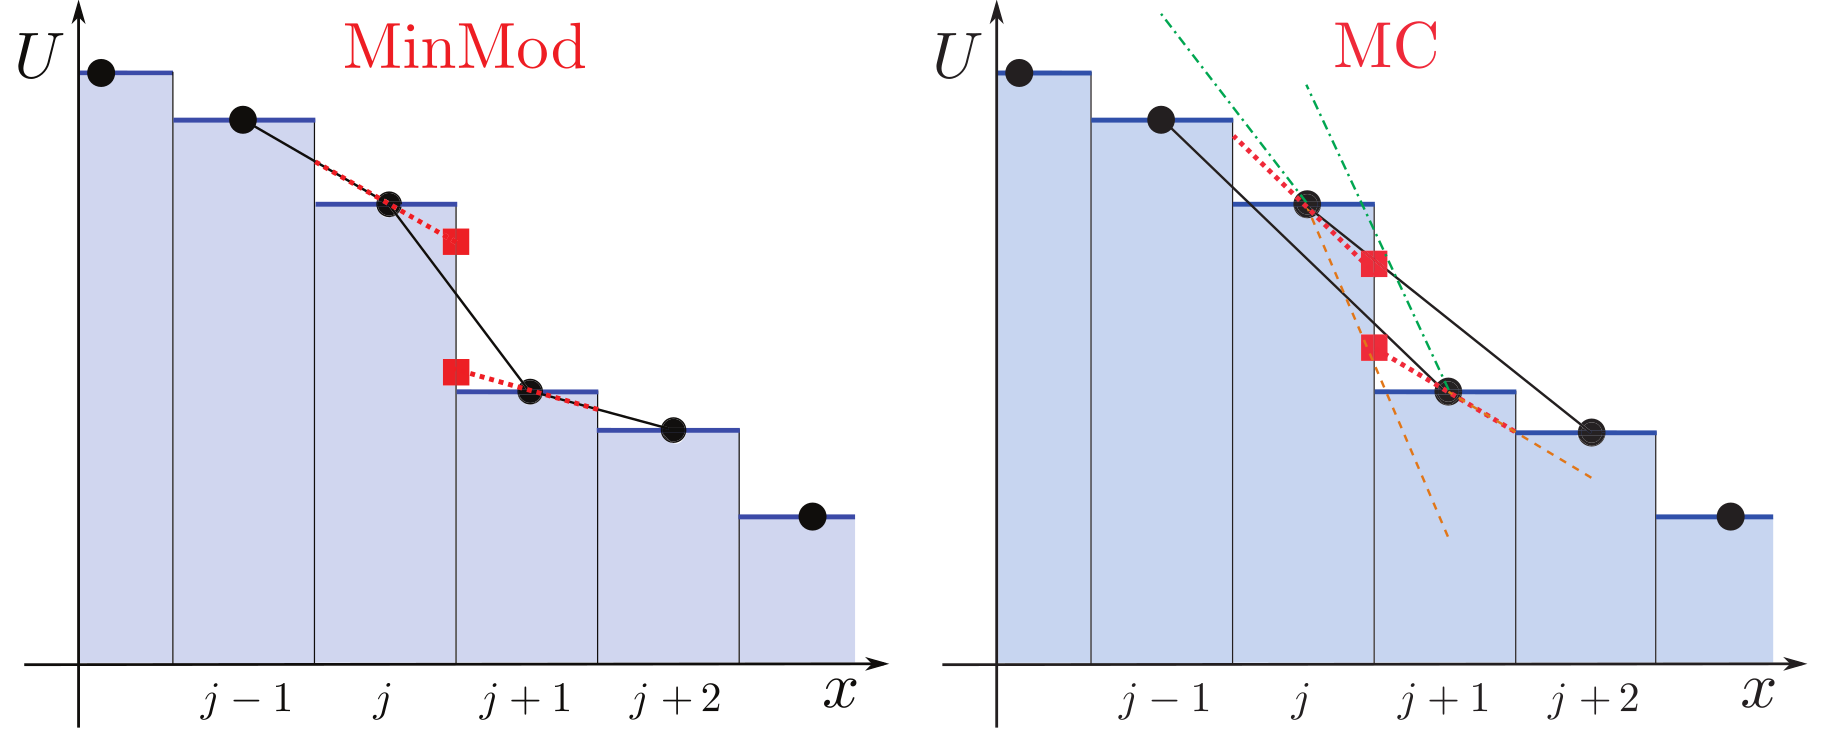
\includegraphics[scale=0.1]{minmod-mc}
        \caption{Minmod and MC Slope Limiters}
\end{figure}
\begin{figure}[h]
        \centering
        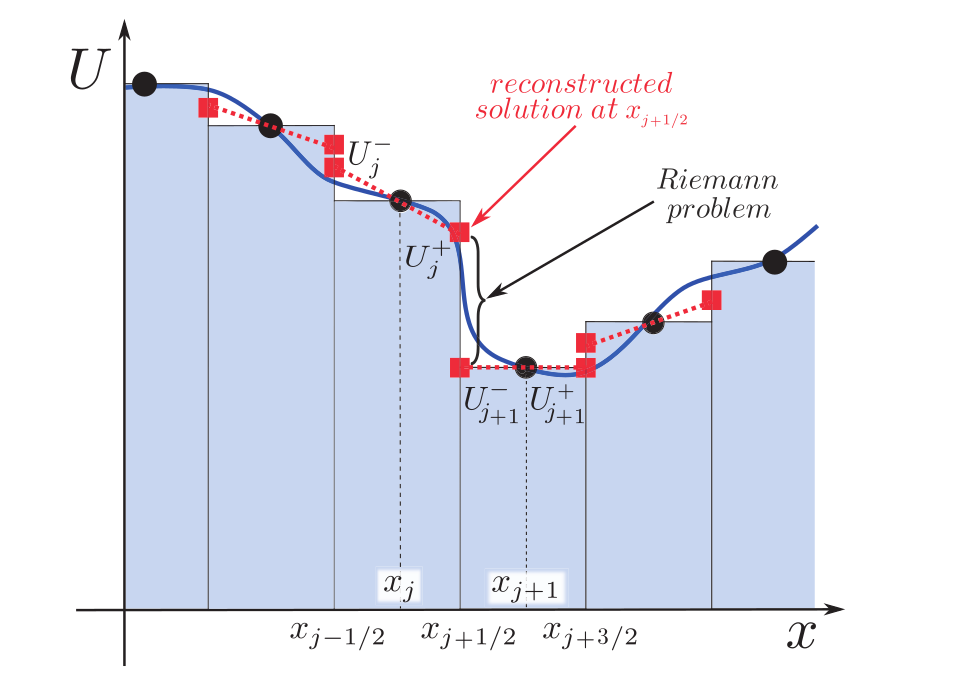
\includegraphics[scale=0.2]{boundary-extrapolated-values}
        \caption{Schematic Representation of Boundary-Extrapolated Values}
\end{figure}
